% Created by tikzDevice version 0.12.6 on 2024-04-08 15:44:13
% !TEX encoding = UTF-8 Unicode
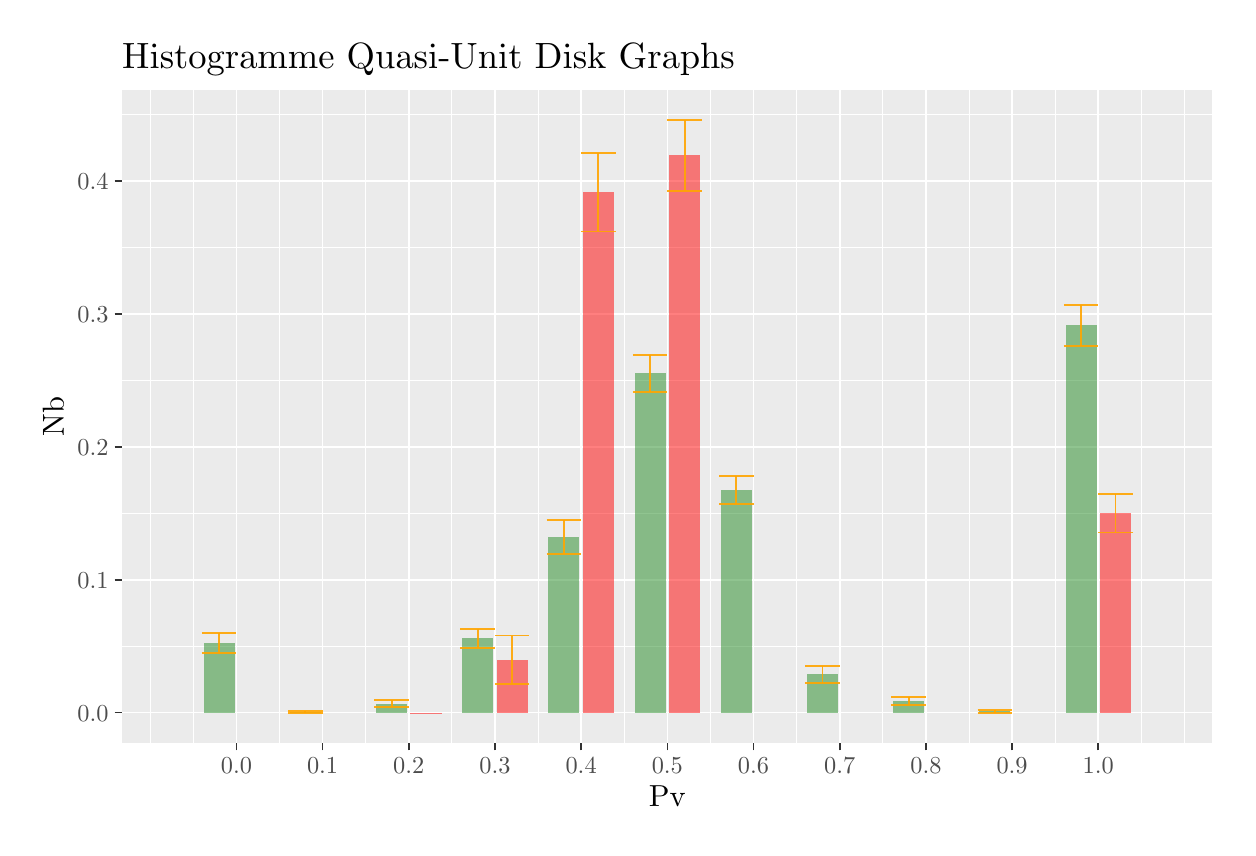
\begin{tikzpicture}[x=1pt,y=1pt]
\definecolor{fillColor}{RGB}{255,255,255}
\path[use as bounding box,fill=fillColor,fill opacity=0.00] (0,0) rectangle (433.62,289.08);
\begin{scope}
\path[clip] (  0.00,  0.00) rectangle (433.62,289.08);
\definecolor{drawColor}{RGB}{255,255,255}
\definecolor{fillColor}{RGB}{255,255,255}

\path[draw=drawColor,line width= 0.6pt,line join=round,line cap=round,fill=fillColor] (  0.00,  0.00) rectangle (433.62,289.08);
\end{scope}
\begin{scope}
\path[clip] ( 34.16, 30.69) rectangle (428.12,266.42);
\definecolor{fillColor}{gray}{0.92}

\path[fill=fillColor] ( 34.16, 30.69) rectangle (428.12,266.42);
\definecolor{drawColor}{RGB}{255,255,255}

\path[draw=drawColor,line width= 0.3pt,line join=round] ( 34.16, 65.59) --
	(428.12, 65.59);

\path[draw=drawColor,line width= 0.3pt,line join=round] ( 34.16,113.64) --
	(428.12,113.64);

\path[draw=drawColor,line width= 0.3pt,line join=round] ( 34.16,161.68) --
	(428.12,161.68);

\path[draw=drawColor,line width= 0.3pt,line join=round] ( 34.16,209.73) --
	(428.12,209.73);

\path[draw=drawColor,line width= 0.3pt,line join=round] ( 34.16,257.78) --
	(428.12,257.78);

\path[draw=drawColor,line width= 0.3pt,line join=round] ( 44.28, 30.69) --
	( 44.28,266.42);

\path[draw=drawColor,line width= 0.3pt,line join=round] ( 59.85, 30.69) --
	( 59.85,266.42);

\path[draw=drawColor,line width= 0.3pt,line join=round] ( 90.99, 30.69) --
	( 90.99,266.42);

\path[draw=drawColor,line width= 0.3pt,line join=round] (122.14, 30.69) --
	(122.14,266.42);

\path[draw=drawColor,line width= 0.3pt,line join=round] (153.28, 30.69) --
	(153.28,266.42);

\path[draw=drawColor,line width= 0.3pt,line join=round] (184.42, 30.69) --
	(184.42,266.42);

\path[draw=drawColor,line width= 0.3pt,line join=round] (215.57, 30.69) --
	(215.57,266.42);

\path[draw=drawColor,line width= 0.3pt,line join=round] (246.71, 30.69) --
	(246.71,266.42);

\path[draw=drawColor,line width= 0.3pt,line join=round] (277.85, 30.69) --
	(277.85,266.42);

\path[draw=drawColor,line width= 0.3pt,line join=round] (309.00, 30.69) --
	(309.00,266.42);

\path[draw=drawColor,line width= 0.3pt,line join=round] (340.14, 30.69) --
	(340.14,266.42);

\path[draw=drawColor,line width= 0.3pt,line join=round] (371.28, 30.69) --
	(371.28,266.42);

\path[draw=drawColor,line width= 0.3pt,line join=round] (402.43, 30.69) --
	(402.43,266.42);

\path[draw=drawColor,line width= 0.3pt,line join=round] (418.00, 30.69) --
	(418.00,266.42);

\path[draw=drawColor,line width= 0.6pt,line join=round] ( 34.16, 41.57) --
	(428.12, 41.57);

\path[draw=drawColor,line width= 0.6pt,line join=round] ( 34.16, 89.61) --
	(428.12, 89.61);

\path[draw=drawColor,line width= 0.6pt,line join=round] ( 34.16,137.66) --
	(428.12,137.66);

\path[draw=drawColor,line width= 0.6pt,line join=round] ( 34.16,185.71) --
	(428.12,185.71);

\path[draw=drawColor,line width= 0.6pt,line join=round] ( 34.16,233.75) --
	(428.12,233.75);

\path[draw=drawColor,line width= 0.6pt,line join=round] ( 75.42, 30.69) --
	( 75.42,266.42);

\path[draw=drawColor,line width= 0.6pt,line join=round] (106.56, 30.69) --
	(106.56,266.42);

\path[draw=drawColor,line width= 0.6pt,line join=round] (137.71, 30.69) --
	(137.71,266.42);

\path[draw=drawColor,line width= 0.6pt,line join=round] (168.85, 30.69) --
	(168.85,266.42);

\path[draw=drawColor,line width= 0.6pt,line join=round] (199.99, 30.69) --
	(199.99,266.42);

\path[draw=drawColor,line width= 0.6pt,line join=round] (231.14, 30.69) --
	(231.14,266.42);

\path[draw=drawColor,line width= 0.6pt,line join=round] (262.28, 30.69) --
	(262.28,266.42);

\path[draw=drawColor,line width= 0.6pt,line join=round] (293.42, 30.69) --
	(293.42,266.42);

\path[draw=drawColor,line width= 0.6pt,line join=round] (324.57, 30.69) --
	(324.57,266.42);

\path[draw=drawColor,line width= 0.6pt,line join=round] (355.71, 30.69) --
	(355.71,266.42);

\path[draw=drawColor,line width= 0.6pt,line join=round] (386.86, 30.69) --
	(386.86,266.42);
\definecolor{fillColor}{RGB}{34,139,34}

\path[fill=fillColor,fill opacity=0.50] ( 63.59, 41.57) rectangle ( 74.80, 66.78);

\path[fill=fillColor,fill opacity=0.50] ( 94.73, 41.57) rectangle (105.94, 41.75);

\path[fill=fillColor,fill opacity=0.50] (125.87, 41.57) rectangle (137.09, 44.83);

\path[fill=fillColor,fill opacity=0.50] (157.02, 41.57) rectangle (168.23, 68.43);

\path[fill=fillColor,fill opacity=0.50] (188.16, 41.57) rectangle (199.37,105.06);

\path[fill=fillColor,fill opacity=0.50] (219.30, 41.57) rectangle (230.52,164.23);

\path[fill=fillColor,fill opacity=0.50] (250.45, 41.57) rectangle (261.66,121.96);

\path[fill=fillColor,fill opacity=0.50] (281.59, 41.57) rectangle (292.80, 55.38);

\path[fill=fillColor,fill opacity=0.50] (312.73, 41.57) rectangle (323.95, 45.76);

\path[fill=fillColor,fill opacity=0.50] (343.88, 41.57) rectangle (355.09, 42.04);

\path[fill=fillColor,fill opacity=0.50] (375.02, 41.57) rectangle (386.23,181.49);
\definecolor{fillColor}{RGB}{255,0,0}

\path[fill=fillColor,fill opacity=0.50] (138.33, 41.57) rectangle (149.54, 41.59);

\path[fill=fillColor,fill opacity=0.50] (169.47, 41.57) rectangle (180.69, 60.63);

\path[fill=fillColor,fill opacity=0.50] (200.62, 41.57) rectangle (211.83,229.57);

\path[fill=fillColor,fill opacity=0.50] (231.76, 41.57) rectangle (242.97,242.89);

\path[fill=fillColor,fill opacity=0.50] (387.48, 41.57) rectangle (398.69,113.61);
\definecolor{drawColor}{RGB}{255,165,0}

\path[draw=drawColor,draw opacity=0.90,line width= 0.7pt,line join=round] ( 62.96, 70.36) --
	( 75.42, 70.36);

\path[draw=drawColor,draw opacity=0.90,line width= 0.7pt,line join=round] ( 69.19, 70.36) --
	( 69.19, 63.19);

\path[draw=drawColor,draw opacity=0.90,line width= 0.7pt,line join=round] ( 62.96, 63.19) --
	( 75.42, 63.19);

\path[draw=drawColor,draw opacity=0.90,line width= 0.7pt,line join=round] ( 94.11, 42.09) --
	(106.56, 42.09);

\path[draw=drawColor,draw opacity=0.90,line width= 0.7pt,line join=round] (100.34, 42.09) --
	(100.34, 41.40);

\path[draw=drawColor,draw opacity=0.90,line width= 0.7pt,line join=round] ( 94.11, 41.40) --
	(106.56, 41.40);

\path[draw=drawColor,draw opacity=0.90,line width= 0.7pt,line join=round] (125.25, 46.12) --
	(137.71, 46.12);

\path[draw=drawColor,draw opacity=0.90,line width= 0.7pt,line join=round] (131.48, 46.12) --
	(131.48, 43.55);

\path[draw=drawColor,draw opacity=0.90,line width= 0.7pt,line join=round] (125.25, 43.55) --
	(137.71, 43.55);

\path[draw=drawColor,draw opacity=0.90,line width= 0.7pt,line join=round] (156.39, 71.77) --
	(168.85, 71.77);

\path[draw=drawColor,draw opacity=0.90,line width= 0.7pt,line join=round] (162.62, 71.77) --
	(162.62, 65.09);

\path[draw=drawColor,draw opacity=0.90,line width= 0.7pt,line join=round] (156.39, 65.09) --
	(168.85, 65.09);

\path[draw=drawColor,draw opacity=0.90,line width= 0.7pt,line join=round] (187.54,111.19) --
	(199.99,111.19);

\path[draw=drawColor,draw opacity=0.90,line width= 0.7pt,line join=round] (193.77,111.19) --
	(193.77, 98.93);

\path[draw=drawColor,draw opacity=0.90,line width= 0.7pt,line join=round] (187.54, 98.93) --
	(199.99, 98.93);

\path[draw=drawColor,draw opacity=0.90,line width= 0.7pt,line join=round] (218.68,170.91) --
	(231.14,170.91);

\path[draw=drawColor,draw opacity=0.90,line width= 0.7pt,line join=round] (224.91,170.91) --
	(224.91,157.56);

\path[draw=drawColor,draw opacity=0.90,line width= 0.7pt,line join=round] (218.68,157.56) --
	(231.14,157.56);

\path[draw=drawColor,draw opacity=0.90,line width= 0.7pt,line join=round] (249.82,127.04) --
	(262.28,127.04);

\path[draw=drawColor,draw opacity=0.90,line width= 0.7pt,line join=round] (256.05,127.04) --
	(256.05,116.89);

\path[draw=drawColor,draw opacity=0.90,line width= 0.7pt,line join=round] (249.82,116.89) --
	(262.28,116.89);

\path[draw=drawColor,draw opacity=0.90,line width= 0.7pt,line join=round] (280.97, 58.37) --
	(293.42, 58.37);

\path[draw=drawColor,draw opacity=0.90,line width= 0.7pt,line join=round] (287.20, 58.37) --
	(287.20, 52.39);

\path[draw=drawColor,draw opacity=0.90,line width= 0.7pt,line join=round] (280.97, 52.39) --
	(293.42, 52.39);

\path[draw=drawColor,draw opacity=0.90,line width= 0.7pt,line join=round] (312.11, 47.24) --
	(324.57, 47.24);

\path[draw=drawColor,draw opacity=0.90,line width= 0.7pt,line join=round] (318.34, 47.24) --
	(318.34, 44.28);

\path[draw=drawColor,draw opacity=0.90,line width= 0.7pt,line join=round] (312.11, 44.28) --
	(324.57, 44.28);

\path[draw=drawColor,draw opacity=0.90,line width= 0.7pt,line join=round] (343.25, 42.48) --
	(355.71, 42.48);

\path[draw=drawColor,draw opacity=0.90,line width= 0.7pt,line join=round] (349.48, 42.48) --
	(349.48, 41.59);

\path[draw=drawColor,draw opacity=0.90,line width= 0.7pt,line join=round] (343.25, 41.59) --
	(355.71, 41.59);

\path[draw=drawColor,draw opacity=0.90,line width= 0.7pt,line join=round] (374.40,188.96) --
	(386.86,188.96);

\path[draw=drawColor,draw opacity=0.90,line width= 0.7pt,line join=round] (380.63,188.96) --
	(380.63,174.01);

\path[draw=drawColor,draw opacity=0.90,line width= 0.7pt,line join=round] (374.40,174.01) --
	(386.86,174.01);

\path[draw=drawColor,draw opacity=0.90,line width= 0.7pt,line join=round] (168.85, 69.43) --
	(181.31, 69.43);

\path[draw=drawColor,draw opacity=0.90,line width= 0.7pt,line join=round] (175.08, 69.43) --
	(175.08, 51.83);

\path[draw=drawColor,draw opacity=0.90,line width= 0.7pt,line join=round] (168.85, 51.83) --
	(181.31, 51.83);

\path[draw=drawColor,draw opacity=0.90,line width= 0.7pt,line join=round] (199.99,243.71) --
	(212.45,243.71);

\path[draw=drawColor,draw opacity=0.90,line width= 0.7pt,line join=round] (206.22,243.71) --
	(206.22,215.43);

\path[draw=drawColor,draw opacity=0.90,line width= 0.7pt,line join=round] (199.99,215.43) --
	(212.45,215.43);

\path[draw=drawColor,draw opacity=0.90,line width= 0.7pt,line join=round] (231.14,255.71) --
	(243.60,255.71);

\path[draw=drawColor,draw opacity=0.90,line width= 0.7pt,line join=round] (237.37,255.71) --
	(237.37,230.08);

\path[draw=drawColor,draw opacity=0.90,line width= 0.7pt,line join=round] (231.14,230.08) --
	(243.60,230.08);

\path[draw=drawColor,draw opacity=0.90,line width= 0.7pt,line join=round] (386.86,120.56) --
	(399.31,120.56);

\path[draw=drawColor,draw opacity=0.90,line width= 0.7pt,line join=round] (393.08,120.56) --
	(393.08,106.67);

\path[draw=drawColor,draw opacity=0.90,line width= 0.7pt,line join=round] (386.86,106.67) --
	(399.31,106.67);
\end{scope}
\begin{scope}
\path[clip] (  0.00,  0.00) rectangle (433.62,289.08);
\definecolor{drawColor}{gray}{0.30}

\node[text=drawColor,anchor=base east,inner sep=0pt, outer sep=0pt, scale=  0.88] at ( 29.21, 38.54) {0.0};

\node[text=drawColor,anchor=base east,inner sep=0pt, outer sep=0pt, scale=  0.88] at ( 29.21, 86.58) {0.1};

\node[text=drawColor,anchor=base east,inner sep=0pt, outer sep=0pt, scale=  0.88] at ( 29.21,134.63) {0.2};

\node[text=drawColor,anchor=base east,inner sep=0pt, outer sep=0pt, scale=  0.88] at ( 29.21,182.68) {0.3};

\node[text=drawColor,anchor=base east,inner sep=0pt, outer sep=0pt, scale=  0.88] at ( 29.21,230.72) {0.4};
\end{scope}
\begin{scope}
\path[clip] (  0.00,  0.00) rectangle (433.62,289.08);
\definecolor{drawColor}{gray}{0.20}

\path[draw=drawColor,line width= 0.6pt,line join=round] ( 31.41, 41.57) --
	( 34.16, 41.57);

\path[draw=drawColor,line width= 0.6pt,line join=round] ( 31.41, 89.61) --
	( 34.16, 89.61);

\path[draw=drawColor,line width= 0.6pt,line join=round] ( 31.41,137.66) --
	( 34.16,137.66);

\path[draw=drawColor,line width= 0.6pt,line join=round] ( 31.41,185.71) --
	( 34.16,185.71);

\path[draw=drawColor,line width= 0.6pt,line join=round] ( 31.41,233.75) --
	( 34.16,233.75);
\end{scope}
\begin{scope}
\path[clip] (  0.00,  0.00) rectangle (433.62,289.08);
\definecolor{drawColor}{gray}{0.20}

\path[draw=drawColor,line width= 0.6pt,line join=round] ( 75.42, 27.94) --
	( 75.42, 30.69);

\path[draw=drawColor,line width= 0.6pt,line join=round] (106.56, 27.94) --
	(106.56, 30.69);

\path[draw=drawColor,line width= 0.6pt,line join=round] (137.71, 27.94) --
	(137.71, 30.69);

\path[draw=drawColor,line width= 0.6pt,line join=round] (168.85, 27.94) --
	(168.85, 30.69);

\path[draw=drawColor,line width= 0.6pt,line join=round] (199.99, 27.94) --
	(199.99, 30.69);

\path[draw=drawColor,line width= 0.6pt,line join=round] (231.14, 27.94) --
	(231.14, 30.69);

\path[draw=drawColor,line width= 0.6pt,line join=round] (262.28, 27.94) --
	(262.28, 30.69);

\path[draw=drawColor,line width= 0.6pt,line join=round] (293.42, 27.94) --
	(293.42, 30.69);

\path[draw=drawColor,line width= 0.6pt,line join=round] (324.57, 27.94) --
	(324.57, 30.69);

\path[draw=drawColor,line width= 0.6pt,line join=round] (355.71, 27.94) --
	(355.71, 30.69);

\path[draw=drawColor,line width= 0.6pt,line join=round] (386.86, 27.94) --
	(386.86, 30.69);
\end{scope}
\begin{scope}
\path[clip] (  0.00,  0.00) rectangle (433.62,289.08);
\definecolor{drawColor}{gray}{0.30}

\node[text=drawColor,anchor=base,inner sep=0pt, outer sep=0pt, scale=  0.88] at ( 75.42, 19.68) {0.0};

\node[text=drawColor,anchor=base,inner sep=0pt, outer sep=0pt, scale=  0.88] at (106.56, 19.68) {0.1};

\node[text=drawColor,anchor=base,inner sep=0pt, outer sep=0pt, scale=  0.88] at (137.71, 19.68) {0.2};

\node[text=drawColor,anchor=base,inner sep=0pt, outer sep=0pt, scale=  0.88] at (168.85, 19.68) {0.3};

\node[text=drawColor,anchor=base,inner sep=0pt, outer sep=0pt, scale=  0.88] at (199.99, 19.68) {0.4};

\node[text=drawColor,anchor=base,inner sep=0pt, outer sep=0pt, scale=  0.88] at (231.14, 19.68) {0.5};

\node[text=drawColor,anchor=base,inner sep=0pt, outer sep=0pt, scale=  0.88] at (262.28, 19.68) {0.6};

\node[text=drawColor,anchor=base,inner sep=0pt, outer sep=0pt, scale=  0.88] at (293.42, 19.68) {0.7};

\node[text=drawColor,anchor=base,inner sep=0pt, outer sep=0pt, scale=  0.88] at (324.57, 19.68) {0.8};

\node[text=drawColor,anchor=base,inner sep=0pt, outer sep=0pt, scale=  0.88] at (355.71, 19.68) {0.9};

\node[text=drawColor,anchor=base,inner sep=0pt, outer sep=0pt, scale=  0.88] at (386.86, 19.68) {1.0};
\end{scope}
\begin{scope}
\path[clip] (  0.00,  0.00) rectangle (433.62,289.08);
\definecolor{drawColor}{RGB}{0,0,0}

\node[text=drawColor,anchor=base,inner sep=0pt, outer sep=0pt, scale=  1.10] at (231.14,  7.64) {Pv};
\end{scope}
\begin{scope}
\path[clip] (  0.00,  0.00) rectangle (433.62,289.08);
\definecolor{drawColor}{RGB}{0,0,0}

\node[text=drawColor,rotate= 90.00,anchor=base,inner sep=0pt, outer sep=0pt, scale=  1.10] at ( 13.08,148.55) {Nb};
\end{scope}
\begin{scope}
\path[clip] (  0.00,  0.00) rectangle (433.62,289.08);
\definecolor{drawColor}{RGB}{0,0,0}

\node[text=drawColor,anchor=base west,inner sep=0pt, outer sep=0pt, scale=  1.32] at ( 34.16,274.49) {Histogramme Quasi-Unit Disk Graphs};
\end{scope}
\end{tikzpicture}
